% second should be about how ppl usually take care of generaliztion : last layer, whole fine tunning, domain generalizaiton .... but they need a lot of data. How come radiologist have descriptive model and interptrable models and it works so well and doesn't need that much data b/c they rely on some invariant description of the disease
% 1:06
% third paragraph (interpretbale models): there several class of interptrable models. We focus on one based on human understable concepts, there several of those too but they are not good in term of performance

% so do you see what I am doing with each paragraph in intro?





% 1:09
% I try to end it what I am going to tell them in the next parag

% What is the problem and why people care

Model generalizability is one of the main challenges of AI, exceptionally in high stake applications such as healthcare. While Neural Networks (NN) have achieved state-of-the-art (SOTA) performance in many applications such as disease classification~\cite{irvin2019chexpert}, they are brittle to small shifts in the distribution~\cite{guan2021domain} caused by a change in acquisition protocol or scanner type. Fine-tuning a model on the target domain can alleviate this problem, but that requires a substantial amount of labeled data. On the contrary, to read abnormality from an image, radiologists usually follow descriptive rules that are reasonably generalizable. We develop a method to extract a mixture of interpretable models based on visual concepts, similar to radiologists' rule, from a pre-trained NN. Such a model is more efficient in computing and data than the original model for fine-tuning to a new distribution.




% Existing domain adaption methods in medical imaging either rely on transfer learning \ie finetuning the model with the target data~\cite{zhang2019unsupervised, swati2019brain, kaur2019improving, wang2017balanced, kumar2017cross}, or aligning features~\cite{karani2018lifelong, guan2020attention, gao2019decoding} or data augmentation~\cite{gholami2019novel}. However, significant computation costs and extensive training data in the target domain are necessary to transfer these models across domains. Also, NN are Blackboxes (BB), offering limited interpretability. Nonetheless, a radiologist predicts a disease using invariant interpretable rules involving anatomical and observation concepts which are generalizable across domains. These rules can be intervened or modified based according to circumstances. We assume that the explainable component of a BB can be approximated with an interpretable model.

Many factors contribute to changes in the distribution of data in medical images. These can include changes in acquisition protocol, and variations in scanner build [cite]. When it comes to adapting a neural network trained on one setting to a new domain, one approach is to fine-tune the whole or part of the network [cite]. However, this can require a significant amount of labeled data and can be computationally expensive [cite]. On the other hand, radiologists search for patterns of changes in anatomy and apply logical rules based on their observations to rule out certain diagnoses. This approach is transparent and closer to an interpretable-by-design approach in AI.

% For example, modern interpretable methods highlight human understandable \emph{concepts} that contribute to the downstream prediction.

% Interpretable models also have a long history in statistics and machine learning~\cite{letham2015interpretable, breiman1984classification}. 
% Early interpretable models are primarily designed for tabular data~\cite{hastie1987generalized, letham2015interpretable, breiman1984classification}. 
% Modern inherently interpretable models \eg Concept Bottleneck Models~\cite{koh2020concept}, Antehoc Concept Bottlenecks~\cite{sarkar2021inducing}, Concept Embedding Models~\cite{zarlenga2022concept} in vision first predict the humanly understandable \emph{concepts} from the input images, followed by labels from the concepts. Recently Posthoc Concept Bottleneck models (PCBMs) ~\cite{yuksekgonul2022post} identify concepts from the embeddings of BB. All these methods rely on a single interpretable classifier to explain the entire dataset, unable to capture the diverse sample-specific explanations and abysmal performance. Also, they are limited to computer vision datasets.

There are many variants of NN that are interpretable by design [cite-cynthia]. Standard methods find an interpretable function (\eg linear regression or rule-based method) between human-understandable concepts and final output [cite]. A concept classifier is used to detect the presence or absence of concepts in an image. Different variants of these approaches have been proposed [cite,cite] and used for medical imaging purposes [cite-several medical imaging]. Recently Posthoc Concept Bottleneck models (PCBMs) ~\cite{yuksekgonul2022post} identify concepts from the embeddings of BB, although not in the medical imaging domain. To the best of our knowledge, the common design choice amongst those methods relies on a single interpretable classifier to explain the entire dataset, unable to capture the diverse sample-specific explanations and suboptimal performance. 

\begin{figure*}[ht]
\begin{center}
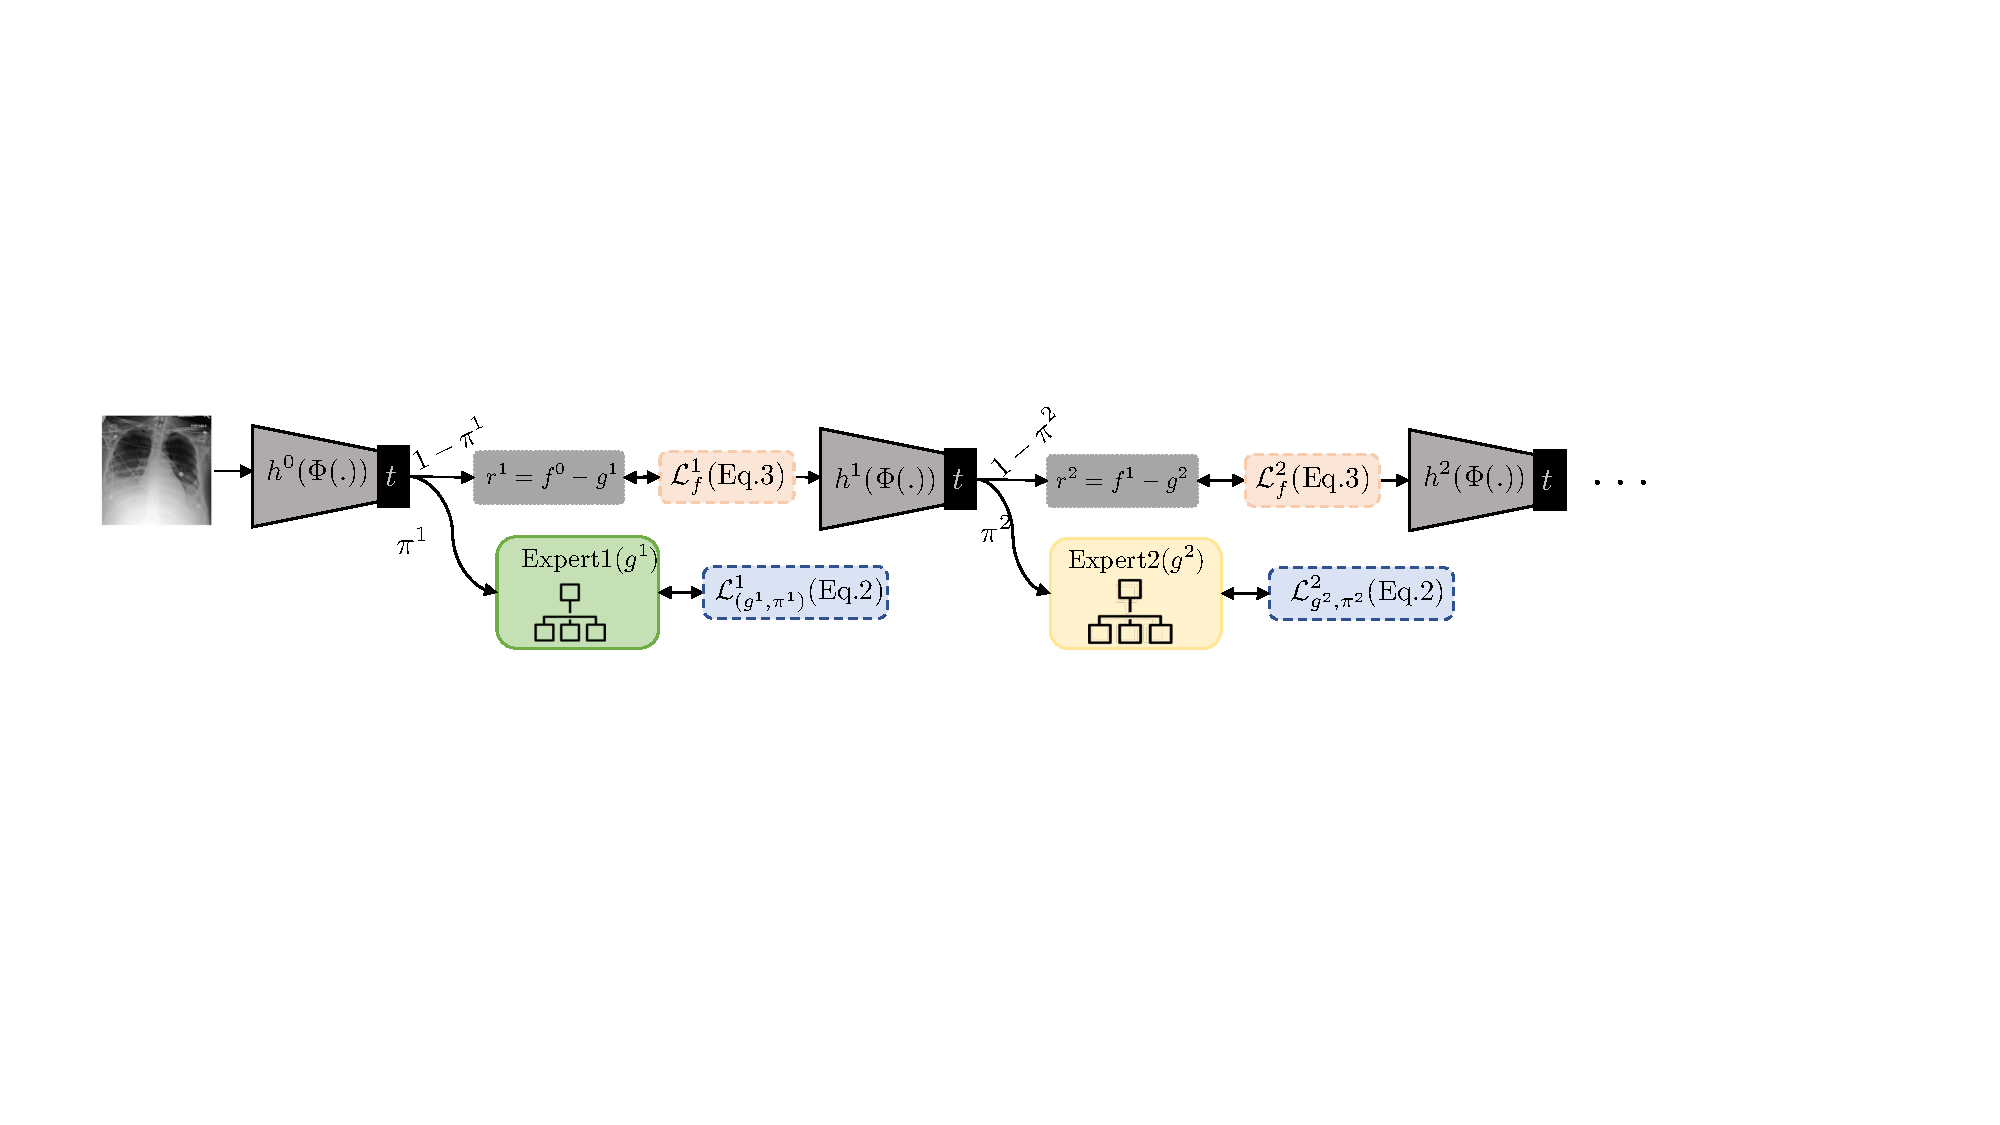
\includegraphics[width=\linewidth]{plots/main/Schematic.pdf}
\caption{Schematic xxxxxxxxx. }
\label{fig:qual}
\end{center}
\end{figure*}

% Recently the Route, Interpret and Repeat (RIR)~\cite{ghosh2023route} algorithm relaxes this assumption by iteratively extracting a mixture of interpretable models and a residual network from the given BB. They name interpretable models in each iteration as experts to offer FOL explanations, specializing in various subsets of data defined by it's  coverage. However, like all concept-based models, RIR is limited to computer vision datasets.

\textbf{Our contributions.}
 In this paper, we propose a novel data-efficient interpretable method to be transferred between two domains. We address the problem of class imbalance in a large medical imaging dataset by estimating the class-stratified coverage by multiplying the fraction of samples within a class by the total data coverage. As the concept annotation is expensive, we assume the target domain lacks concept-level annotation. Hence, we adopt the pseudo labeling from semi-supervised learning~\cite{lee2013pseudo} to learn the concept detector in the target domain and finetune the interpretable models. Our work is the first to apply concept-based methods to CXRs and utilize them to transfer between domains. 
 Our extensive experiments demonstrate that our method (1) is able to capture diverse instance-specific concepts in the FOLs compared to all other interpretable models, (2) does not compromise the performance, (3) is able to identify  ``harder'' samples, (4) can be transferred from source to target domain.
 
 
 
 % Ware the first to apply State-of-the-art (SOTA) concept-based interpretable models to a large CXR dataset. Also, we propose a novel stratified RIR algorithm to cover samples from a specific class to address the class imbalance in a large real-life CXR dataset. We estimate the coverages of positive and negative classes by multiplying the weight of a class with the given coverage. The weights of the class are the proportion of samples from training data. Our extensive experiments using MIMIC-CXR~\cite{12_johnsonmimic} demonstrate that our method is able to capture diverse instance-specific concepts in the FOLs compared to all other interpretable models. We next showcase the importance of the concepts quantitatively (1) by zeroing out them~\cite{ghosh2023route} and (2) during test time intervention~\cite{koh2020concept}. Finally, we hypothesize the concepts to be domain invariant. So we effectively transfer the models trained on MIMIC-CXR to Stanford-CXR~\cite{irvin2019chexpert} with minimal computation cost and limited Stanford-CXR training data.

% FOL is a logical function
% that accepts predicates (concept presence/absent) as input and returns a True/False output being a
% logical expression of the predicates. The logical expression, which is a set of AND, OR, Negative,
% and parenthesis, can be written in the so-called Disjunctive Normal Form (DNF). DNF is a FOL logical formula composed of a disjunction (OR) of conjunctions (AND), known as the ``sum of products''. 
% % Why the solution is smart / Did it work.

% 1. First to use concept bottleneck in CXR
% 2. First to apply CBM to domain transfer